% Options for packages loaded elsewhere
\PassOptionsToPackage{unicode}{hyperref}
\PassOptionsToPackage{hyphens}{url}
\PassOptionsToPackage{dvipsnames,svgnames,x11names}{xcolor}
%
\documentclass[
  letterpaper,
]{report}

\usepackage{amsmath,amssymb}
\usepackage{iftex}
\ifPDFTeX
  \usepackage[T1]{fontenc}
  \usepackage[utf8]{inputenc}
  \usepackage{textcomp} % provide euro and other symbols
\else % if luatex or xetex
  \usepackage{unicode-math}
  \defaultfontfeatures{Scale=MatchLowercase}
  \defaultfontfeatures[\rmfamily]{Ligatures=TeX,Scale=1}
\fi
\usepackage{lmodern}
\ifPDFTeX\else  
    % xetex/luatex font selection
\fi
% Use upquote if available, for straight quotes in verbatim environments
\IfFileExists{upquote.sty}{\usepackage{upquote}}{}
\IfFileExists{microtype.sty}{% use microtype if available
  \usepackage[]{microtype}
  \UseMicrotypeSet[protrusion]{basicmath} % disable protrusion for tt fonts
}{}
\makeatletter
\@ifundefined{KOMAClassName}{% if non-KOMA class
  \IfFileExists{parskip.sty}{%
    \usepackage{parskip}
  }{% else
    \setlength{\parindent}{0pt}
    \setlength{\parskip}{6pt plus 2pt minus 1pt}}
}{% if KOMA class
  \KOMAoptions{parskip=half}}
\makeatother
\usepackage{xcolor}
\setlength{\emergencystretch}{3em} % prevent overfull lines
\setcounter{secnumdepth}{-\maxdimen} % remove section numbering
% Make \paragraph and \subparagraph free-standing
\ifx\paragraph\undefined\else
  \let\oldparagraph\paragraph
  \renewcommand{\paragraph}[1]{\oldparagraph{#1}\mbox{}}
\fi
\ifx\subparagraph\undefined\else
  \let\oldsubparagraph\subparagraph
  \renewcommand{\subparagraph}[1]{\oldsubparagraph{#1}\mbox{}}
\fi

\usepackage{color}
\usepackage{fancyvrb}
\newcommand{\VerbBar}{|}
\newcommand{\VERB}{\Verb[commandchars=\\\{\}]}
\DefineVerbatimEnvironment{Highlighting}{Verbatim}{commandchars=\\\{\}}
% Add ',fontsize=\small' for more characters per line
\usepackage{framed}
\definecolor{shadecolor}{RGB}{241,243,245}
\newenvironment{Shaded}{\begin{snugshade}}{\end{snugshade}}
\newcommand{\AlertTok}[1]{\textcolor[rgb]{0.68,0.00,0.00}{#1}}
\newcommand{\AnnotationTok}[1]{\textcolor[rgb]{0.37,0.37,0.37}{#1}}
\newcommand{\AttributeTok}[1]{\textcolor[rgb]{0.40,0.45,0.13}{#1}}
\newcommand{\BaseNTok}[1]{\textcolor[rgb]{0.68,0.00,0.00}{#1}}
\newcommand{\BuiltInTok}[1]{\textcolor[rgb]{0.00,0.23,0.31}{#1}}
\newcommand{\CharTok}[1]{\textcolor[rgb]{0.13,0.47,0.30}{#1}}
\newcommand{\CommentTok}[1]{\textcolor[rgb]{0.37,0.37,0.37}{#1}}
\newcommand{\CommentVarTok}[1]{\textcolor[rgb]{0.37,0.37,0.37}{\textit{#1}}}
\newcommand{\ConstantTok}[1]{\textcolor[rgb]{0.56,0.35,0.01}{#1}}
\newcommand{\ControlFlowTok}[1]{\textcolor[rgb]{0.00,0.23,0.31}{#1}}
\newcommand{\DataTypeTok}[1]{\textcolor[rgb]{0.68,0.00,0.00}{#1}}
\newcommand{\DecValTok}[1]{\textcolor[rgb]{0.68,0.00,0.00}{#1}}
\newcommand{\DocumentationTok}[1]{\textcolor[rgb]{0.37,0.37,0.37}{\textit{#1}}}
\newcommand{\ErrorTok}[1]{\textcolor[rgb]{0.68,0.00,0.00}{#1}}
\newcommand{\ExtensionTok}[1]{\textcolor[rgb]{0.00,0.23,0.31}{#1}}
\newcommand{\FloatTok}[1]{\textcolor[rgb]{0.68,0.00,0.00}{#1}}
\newcommand{\FunctionTok}[1]{\textcolor[rgb]{0.28,0.35,0.67}{#1}}
\newcommand{\ImportTok}[1]{\textcolor[rgb]{0.00,0.46,0.62}{#1}}
\newcommand{\InformationTok}[1]{\textcolor[rgb]{0.37,0.37,0.37}{#1}}
\newcommand{\KeywordTok}[1]{\textcolor[rgb]{0.00,0.23,0.31}{#1}}
\newcommand{\NormalTok}[1]{\textcolor[rgb]{0.00,0.23,0.31}{#1}}
\newcommand{\OperatorTok}[1]{\textcolor[rgb]{0.37,0.37,0.37}{#1}}
\newcommand{\OtherTok}[1]{\textcolor[rgb]{0.00,0.23,0.31}{#1}}
\newcommand{\PreprocessorTok}[1]{\textcolor[rgb]{0.68,0.00,0.00}{#1}}
\newcommand{\RegionMarkerTok}[1]{\textcolor[rgb]{0.00,0.23,0.31}{#1}}
\newcommand{\SpecialCharTok}[1]{\textcolor[rgb]{0.37,0.37,0.37}{#1}}
\newcommand{\SpecialStringTok}[1]{\textcolor[rgb]{0.13,0.47,0.30}{#1}}
\newcommand{\StringTok}[1]{\textcolor[rgb]{0.13,0.47,0.30}{#1}}
\newcommand{\VariableTok}[1]{\textcolor[rgb]{0.07,0.07,0.07}{#1}}
\newcommand{\VerbatimStringTok}[1]{\textcolor[rgb]{0.13,0.47,0.30}{#1}}
\newcommand{\WarningTok}[1]{\textcolor[rgb]{0.37,0.37,0.37}{\textit{#1}}}

\providecommand{\tightlist}{%
  \setlength{\itemsep}{0pt}\setlength{\parskip}{0pt}}\usepackage{longtable,booktabs,array}
\usepackage{calc} % for calculating minipage widths
% Correct order of tables after \paragraph or \subparagraph
\usepackage{etoolbox}
\makeatletter
\patchcmd\longtable{\par}{\if@noskipsec\mbox{}\fi\par}{}{}
\makeatother
% Allow footnotes in longtable head/foot
\IfFileExists{footnotehyper.sty}{\usepackage{footnotehyper}}{\usepackage{footnote}}
\makesavenoteenv{longtable}
\usepackage{graphicx}
\makeatletter
\def\maxwidth{\ifdim\Gin@nat@width>\linewidth\linewidth\else\Gin@nat@width\fi}
\def\maxheight{\ifdim\Gin@nat@height>\textheight\textheight\else\Gin@nat@height\fi}
\makeatother
% Scale images if necessary, so that they will not overflow the page
% margins by default, and it is still possible to overwrite the defaults
% using explicit options in \includegraphics[width, height, ...]{}
\setkeys{Gin}{width=\maxwidth,height=\maxheight,keepaspectratio}
% Set default figure placement to htbp
\makeatletter
\def\fps@figure{htbp}
\makeatother

\usepackage{titling}
\pretitle{
  \begin{center}
  \huge
  
\includegraphics[width=4cm,height=6cm]{psulogo2.jpg}\\[\bigskipamount]
}
\posttitle{\end{center}}
\posttitle{\end{center}}
\usepackage{booktabs}
\usepackage{longtable}
\usepackage{array}
\usepackage{multirow}
\usepackage{wrapfig}
\usepackage{float}
\usepackage{colortbl}
\usepackage{pdflscape}
\usepackage{tabu}
\usepackage{threeparttable}
\usepackage{xcolor}
\usepackage{soul}
\usepackage{graphicx}
\usepackage{fancyhdr}
\pagestyle{fancy}
\rhead{
\includegraphics[width = .05\textwidth]{psulogo2.jpg}}
\makeatletter
\makeatother
\makeatletter
\makeatother
\makeatletter
\@ifpackageloaded{caption}{}{\usepackage{caption}}
\AtBeginDocument{%
\ifdefined\contentsname
  \renewcommand*\contentsname{Table of contents}
\else
  \newcommand\contentsname{Table of contents}
\fi
\ifdefined\listfigurename
  \renewcommand*\listfigurename{List of Figures}
\else
  \newcommand\listfigurename{List of Figures}
\fi
\ifdefined\listtablename
  \renewcommand*\listtablename{List of Tables}
\else
  \newcommand\listtablename{List of Tables}
\fi
\ifdefined\figurename
  \renewcommand*\figurename{Figure}
\else
  \newcommand\figurename{Figure}
\fi
\ifdefined\tablename
  \renewcommand*\tablename{Table}
\else
  \newcommand\tablename{Table}
\fi
}
\@ifpackageloaded{float}{}{\usepackage{float}}
\floatstyle{ruled}
\@ifundefined{c@chapter}{\newfloat{codelisting}{h}{lop}}{\newfloat{codelisting}{h}{lop}[chapter]}
\floatname{codelisting}{Listing}
\newcommand*\listoflistings{\listof{codelisting}{List of Listings}}
\makeatother
\makeatletter
\@ifpackageloaded{caption}{}{\usepackage{caption}}
\@ifpackageloaded{subcaption}{}{\usepackage{subcaption}}
\makeatother
\makeatletter
\@ifpackageloaded{tcolorbox}{}{\usepackage[skins,breakable]{tcolorbox}}
\makeatother
\makeatletter
\@ifundefined{shadecolor}{\definecolor{shadecolor}{rgb}{.97, .97, .97}}
\makeatother
\makeatletter
\makeatother
\makeatletter
\makeatother
\ifLuaTeX
  \usepackage{selnolig}  % disable illegal ligatures
\fi
\IfFileExists{bookmark.sty}{\usepackage{bookmark}}{\usepackage{hyperref}}
\IfFileExists{xurl.sty}{\usepackage{xurl}}{} % add URL line breaks if available
\urlstyle{same} % disable monospaced font for URLs
\hypersetup{
  pdftitle={Project Name Here},
  pdfauthor={First Member's Name; Second Member's Name; Third Member's Name; Fourth Member's Name},
  colorlinks=true,
  linkcolor={blue},
  filecolor={Maroon},
  citecolor={Blue},
  urlcolor={Blue},
  pdfcreator={LaTeX via pandoc}}

\title{Project Name Here}
\usepackage{etoolbox}
\makeatletter
\providecommand{\subtitle}[1]{% add subtitle to \maketitle
  \apptocmd{\@title}{\par {\large #1 \par}}{}{}
}
\makeatother
\subtitle{CADES Consulting Lab}
\author{First Member's Name \and Second Member's Name \and Third
Member's Name \and Fourth Member's Name}
\date{2023-05-04}

\begin{document}
\maketitle
\ifdefined\Shaded\renewenvironment{Shaded}{\begin{tcolorbox}[frame hidden, boxrule=0pt, borderline west={3pt}{0pt}{shadecolor}, interior hidden, enhanced, sharp corners, breakable]}{\end{tcolorbox}}\fi

\renewcommand*\contentsname{Table of contents}
{
\hypersetup{linkcolor=}
\setcounter{tocdepth}{2}
\tableofcontents
}
\hypertarget{project-report}{%
\chapter{Project Report}\label{project-report}}

To be able to compile this template from R you'll need to follow the
instructions \href{https://quarto.org/docs/get-started/}{here}, where
they explain how to install Quarto, and download the necessary R
packages. You also need to install a distribution of LaTeX by typing in
the \textsf{Terminal} window in \textsf{RStudio} the following command:

\begin{Shaded}
\begin{Highlighting}[]
\NormalTok{quarto install tool tinytex}
\end{Highlighting}
\end{Shaded}

For more details, go over the \textsf{Authoring} tutorial
\href{https://quarto.org/docs/get-started/authoring/rstudio.html}{here}.

\hypertarget{executive-summary}{%
\section{Executive Summary}\label{executive-summary}}

The executive summary contains a brief account of your final
recommendations, it should be very short and to the point. Write the
results not the description of the problem.

\hypertarget{introduction-and-background}{%
\section{Introduction and
Background}\label{introduction-and-background}}

In this section, get right to describing the main questions to be
answered and the goals behind the consulting project taken on. Here
you'll paraphrase the problem you that you tackled, relevant issues
present in the analysis that will be dealt with. You will discuss
relevant background information here, such as some information alluding
to the context of the problem, what the client or other people ion their
field has attempted to solve it, etc. Also, define any technical terms
needed for the remainder of the paper.Don't include technical terms if
you don't use them later. That hurts clarity. Finally, it's a good idea
to summarize your strategy and recommendations in this section, so that
clients will know what to look for as they read.

\hypertarget{data}{%
\section{Data}\label{data}}

\hypertarget{basic-data-description}{%
\subsection{Basic Data Description}\label{basic-data-description}}

Here you should describe how the data were collected; describe the
variables used in the models; number of observations available; and,
discuss issues such as missing data or confidentiality restrictions on
the data. Never include the actual data in the report!!!

\hypertarget{exploratory-data-analysis}{%
\subsection{Exploratory Data Analysis}\label{exploratory-data-analysis}}

It's good practice to carry out a thoughtful exploratory analysis and
provide a succinct description of the results stemming from it.

\hypertarget{connect-the-dots}{%
\subsection{Connect the dots}\label{connect-the-dots}}

In this section, connect the dots for the client so they can get a big
picture idea of how issues and aspects present in their data impact
their ability to solve their question, and help identify suitable
methods to tackle them.

\hypertarget{connect-the-dots-1}{%
\subsection{Connect the Dots}\label{connect-the-dots-1}}

\hypertarget{methods}{%
\section{Methods}\label{methods}}

Here you describe the methodology/methodologies you considered in
exploring the consulting project. Furthermore, you need to state upfront
the assumptions that you are making.

\hypertarget{conclusions-and-recommendations}{%
\section{Conclusions and
recommendations}\label{conclusions-and-recommendations}}

In this section, you discuss your recommended strategy for approaching
the problem and show the specific methods you'd use for in analysis.
Explain what these methods will do in terms of the questions the client
posed and goals of the project. You can discuss issues that merit
further exploration, interesting relationships among variables that are
not quite central to answering the questions that might be things the
client could look into. Importantly mention reservations about the
analyses that you think may require more complex modeling, either due to
modeling assumptions not holding, or by discoveries made along the
process of analyzing the data that might hinder the validity of your
conclusions. Also include any relavant diagnostics for your suggested
methods. Working out a toy example from start to finish is a great way
to demonstrate how your suggested method(s) could be implimented.

\hypertarget{references}{%
\section{References}\label{references}}

Include all bibliographical references used here. See
\href{https://quarto.org/docs/get-started/authoring/rstudio.html\#citations}{this
link} to learn about adding references to the document.

\hypertarget{quarto-basics}{%
\chapter{Quarto Basics}\label{quarto-basics}}

The sections that follow describe a few basic tips on how to use Quarto.
Quarto enables you to weave together content and executable code into a
finished document. To learn more about Quarto see
\url{https://quarto.org}.

See
\href{https://quarto.org/docs/get-started/authoring/rstudio.html}{this
link} to learn more (e.g., cross-references, equations, output formats,
etc.) about authoring documents on Quarto.

\hypertarget{running-code}{%
\section{Running Code}\label{running-code}}

When you click the \textbf{Render} button a document will be generated
that includes both content and the output of embedded code. You can
embed code like this:

\begin{Shaded}
\begin{Highlighting}[]
\DecValTok{1} \SpecialCharTok{+} \DecValTok{1}
\end{Highlighting}
\end{Shaded}

\begin{verbatim}
[1] 2
\end{verbatim}

\begin{Shaded}
\begin{Highlighting}[]
\FunctionTok{summary}\NormalTok{(cars)}
\end{Highlighting}
\end{Shaded}

\begin{verbatim}
     speed           dist       
 Min.   : 4.0   Min.   :  2.00  
 1st Qu.:12.0   1st Qu.: 26.00  
 Median :15.0   Median : 36.00  
 Mean   :15.4   Mean   : 42.98  
 3rd Qu.:19.0   3rd Qu.: 56.00  
 Max.   :25.0   Max.   :120.00  
\end{verbatim}

You can add options to executable code like this

\begin{verbatim}
[1] 4
\end{verbatim}

The \texttt{echo:\ false} option disables the printing of code (only
output is displayed).

\hypertarget{including-plots}{%
\section{Including Plots}\label{including-plots}}

You can also embed plots, for example:

\begin{figure}

{\centering 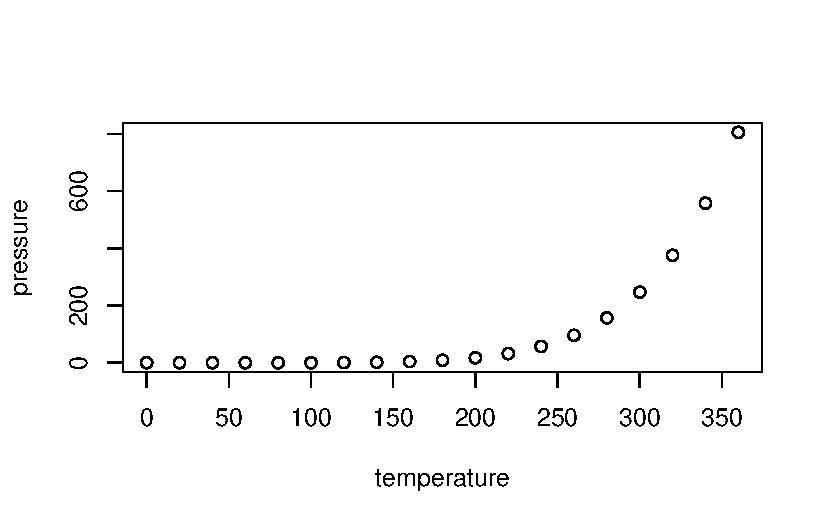
\includegraphics{ReportTemplate_files/figure-pdf/pressure-1.pdf}

}

\end{figure}

Note that the \texttt{echo\ =\ FALSE} parameter was added to the code
chunk to prevent printing of the R code that generated the plot.

\hypertarget{including-tables}{%
\section{Including Tables}\label{including-tables}}

Here's an example of a table

\begin{Shaded}
\begin{Highlighting}[]
\FunctionTok{library}\NormalTok{(knitr)}

\CommentTok{\# Example data}
\NormalTok{headers }\OtherTok{\textless{}{-}} \FunctionTok{c}\NormalTok{(}\StringTok{"Column 1"}\NormalTok{, }\StringTok{"Column 2"}\NormalTok{, }\StringTok{"Column 3"}\NormalTok{)}
\NormalTok{data }\OtherTok{\textless{}{-}} \FunctionTok{data.frame}\NormalTok{(}
  \AttributeTok{a =} \FunctionTok{c}\NormalTok{(}\DecValTok{1}\NormalTok{, }\DecValTok{2}\NormalTok{, }\DecValTok{3}\NormalTok{),}
  \AttributeTok{b =} \FunctionTok{c}\NormalTok{(}\DecValTok{4}\NormalTok{, }\DecValTok{5}\NormalTok{, }\DecValTok{6}\NormalTok{),}
  \AttributeTok{c =} \FunctionTok{c}\NormalTok{(}\DecValTok{7}\NormalTok{, }\DecValTok{8}\NormalTok{, }\DecValTok{9}\NormalTok{)}
\NormalTok{)}

\CommentTok{\# Create the table}
\FunctionTok{kable}\NormalTok{(data, }\AttributeTok{col.names =}\NormalTok{ headers, }\AttributeTok{align =} \FunctionTok{rep}\NormalTok{(}\StringTok{"l"}\NormalTok{, }\FunctionTok{length}\NormalTok{(headers)), }
      \AttributeTok{col.width =} \FunctionTok{rep}\NormalTok{(}\FloatTok{1.5}\NormalTok{, }\FunctionTok{length}\NormalTok{(headers)))}
\end{Highlighting}
\end{Shaded}

\begin{longtable}[]{@{}lll@{}}
\toprule\noalign{}
Column 1 & Column 2 & Column 3 \\
\midrule\noalign{}
\endhead
\bottomrule\noalign{}
\endlastfoot
1 & 4 & 7 \\
2 & 5 & 8 \\
3 & 6 & 9 \\
\end{longtable}



\end{document}
